% ============================================================
%  EXPERIMENT 1 — MAIN SECTIONS  (revised 2026-06-16)
%  Requires: \usepackage{booktabs, multirow, amsmath, graphicx,
%             xcolor, array}
% ============================================================

% ------------------------------------------------------------------
\section{Experiment 1: Coherent Updating in Prospective Forecasts}
\label{sec:exp1}
% ------------------------------------------------------------------

We evaluate whether forecasting agents maintain event-specific causal models that support
coherent updating, using unresolved real-world prediction markets where final outcomes are
not yet known at elicitation time.  This rules out direct outcome memorization
\citep{zou2022forecasting,halawi2024approaching} while preserving the messy evidence
structure of real forecasting: agents must reason about institutions, actors, timelines,
incentives, and latent constraints.  In the hierarchy of
Section~\ref{sec:forecasting-as-inductive} this is the \emph{coherence} rung---the most
demanding test applicable to unresolved markets, and a necessary condition for inductive
world modeling: an agent whose stated hypotheses, evidence updates, and final forecast do
not agree within a case cannot be said to carry a usable event model of it.

The diagnostic logic is simple.  If an agent has a coherent event model, evidence bearing
causally on the yes-resolution hypothesis $H_1$ should move both its stated $P(H_1)$ and
its final forecast in the corresponding direction, while topically adjacent but causally
unrelated evidence should produce little or no movement.  This gives each shortcut account
of Section~\ref{sec:forecasting-as-inductive} a falsifiable signature: surface-feature
matching would move the forecast under irrelevant evidence; post-hoc rationalization
\citep{turpin2023language} would decouple the hypothesis update from the headline forecast;
and market imitation would tie the forecast to the prevailing price.  An agent governed by
any of these should fail at least one check.

\subsection{Markets and agents}
\label{sec:markets-agents}

\textbf{Market pool.}  From the Polymarket API\footnote{\url{https://polymarket.com}} we
retain binary markets that, as of the June~2026 sampling date, are open (unresolved),
resolve within 14--180~days, carry at least 1{,}000 CLOB transactions, and fall in
Politics, Government, Elections, Economics, or Geopolitics.  From this pool we draw
\textbf{100~markets}, maximizing joint diversity across category, mid-price, and topic type
so that no single domain or probability stratum dominates (the Qwen family is additionally
run on a 20-market extension; per-agent market and record counts are in
Appendix~\ref{app:extended-results}).

\textbf{Agents.}  We evaluate \textbf{ten agents} in two tiers.  Three \emph{frontier API
models}---GPT-5.4, Claude Opus~4.8, and DeepSeek V4-Pro---are served via Azure AI~Foundry
with native, Bing-backed web search and run a multi-turn loop (event model, web research,
an optional steelman, and a final structured forecast).  Seven \emph{local open-weight
models}---Qwen~2.5 (7B--72B) \citep{qwen2025qwen25} and Llama (3.1-8B, 3.1-70B, 3.3-70B)
\citep{grattafiori2024llama}---are served via Ollama and retrieve through an explicit
Tavily tool-calling loop.  Because small (7--8B) models frequently fail to invoke tools
when instructed, three searches are pre-executed and injected before synthesis, with up to
three more on request.

\textbf{Forecasts and counterfactual updates.}  Each market--agent cell yields a structured
forecast: a causal event model with key actors and latent variables, hypotheses $H_1$~(YES)
and $H_2$~(NO) with prior and posterior probabilities, and a scalar forecast $\hat{p}$
constrained to equal $P(H_1)$; we run $k=5$ times with independent seeds and summarize by
the median.  We then generate nine synthetic counterfactual evidence packets per market
(three pro-$H_1$, three anti-$H_1$, three orthogonal), pair each with each of the $k$ runs
($9k=45$ records per cell), and have the agent revise its forecast \textbf{with web search
disabled}, so revisions are driven only by the injected evidence.  Full prompts, the packet
taxonomy, and per-stage detail are in Appendix~\ref{app:exp1}.

\textbf{Consistency metrics.}  From the updated forecasts we compute three binary
consistency indicators and one selectivity ratio, adapting directional behavioral tests
\citep{ribeiro2020beyond} and consistency evaluation \citep{elazar2021measuring} to
forecasting (formal definitions in Appendix~\ref{app:metrics}).
\emph{Evidence--Hypothesis Consistency} (EHC) asks whether the posterior $P(H_1)$ moves in
the intended direction after directional evidence; \emph{Hypothesis--Forecast Consistency}
(HFC) asks whether the headline $\hat{p}$ moves likewise; and the \emph{Internal Coherence
Score} (ICS) asks whether the structural invariant $\hat{p}=P(H_1)$ is preserved after
updating.  The \emph{sensitivity ratio}---mean absolute revision under directional evidence
divided by the same under orthogonal evidence---measures causal selectivity: values near
one indicate evidence-insensitive updating, larger values a preferential response to
causally relevant evidence.

\subsection{Results}
\label{sec:exp1-results}

\begin{figure}[t]
\centering
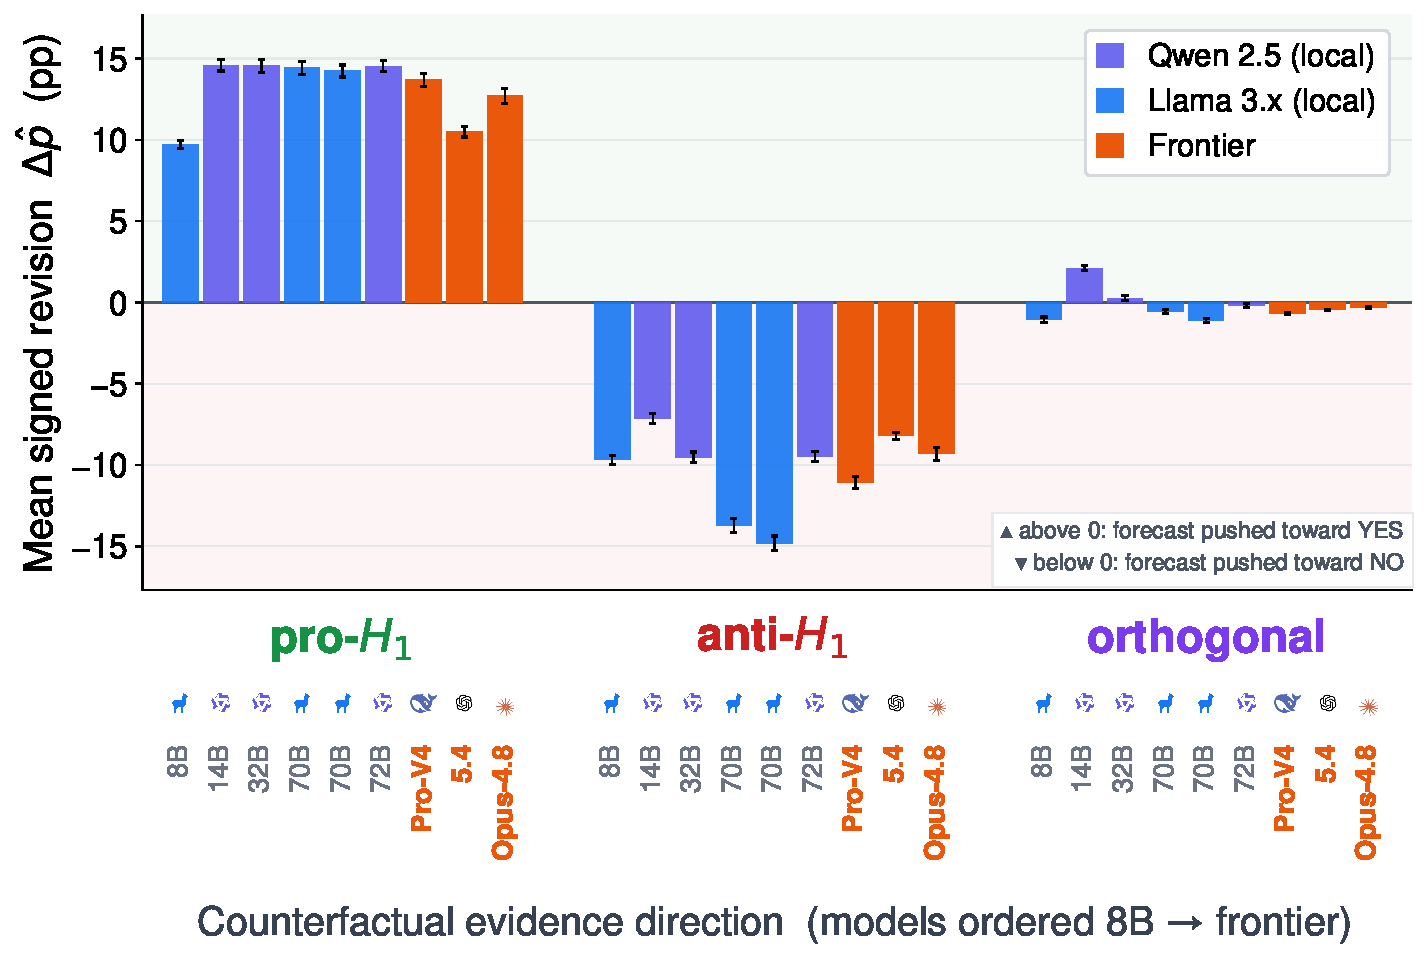
\includegraphics[width=\linewidth]{figures/exp1_direction_selective_updating.pdf}
\caption{
\textbf{Direction-selective updating across ten models and ${\approx}39{,}000$ update
records.}
Mean \emph{signed} forecast revision $\Delta\hat{p}$ (percentage points) after a counterfactual
evidence packet, by evidence direction and agent; within each group models are ordered
$7$B\,$\rightarrow$\,frontier and coloured by family, with $\pm1$~SE error bars.
Evidence built to support the yes-hypothesis (pro-$H_1$) moves the forecast \emph{up}, matched
anti-$H_1$ evidence moves it symmetrically \emph{down}, and causally unrelated (orthogonal)
evidence leaves it essentially unchanged (${\approx}0$~pp)---the signature of updating that
tracks the causal content of the evidence rather than its mere presence. Directional revisions
are large for every model (${\approx}8$--$14$~pp for the frontier agents, orange); what scales is
the orthogonal null, which shrinks toward zero with model size, so causal selectivity improves
with scale (Table~\ref{tab:consistency}).}
\label{fig:exp1-results}
\end{figure}

Table~\ref{tab:consistency} reports the three consistency metrics, the sensitivity ratio,
and the market-association statistics for all ten models.  The results organise around
three main findings.

\begin{table*}[t]
\centering
\caption{Internal consistency, causal sensitivity, and market association by agent,
ordered by decreasing EHC within tier.
EHC and HFC count directional threshold-crossing updates ($|\Delta| \geq 3$\,pp);
ICS counts all records.  Sensitivity is the ratio of mean directional to mean
orthogonal absolute revision (Eq.~\ref{eq:sensitivity}).
$\rho$ is the Spearman rank correlation between the agent's initial forecast and the
Polymarket mid-price and $\overline{|A{-}M|}$ the mean absolute divergence from it---a
market-association control, not calibration (markets are unresolved, so the mid-price is a
proxy, not ground truth); $\bar{\sigma}_k$ is the mean intra-market $k$-run standard
deviation of initial forecasts.  Standard errors for the consistency averages are
$\leq 0.016$.}
\label{tab:consistency}
\small
\begin{tabular}{llcccccccc}
\toprule
\textbf{Model} & \textbf{Type}
  & \textbf{EHC}\,$\uparrow$ & \textbf{HFC}\,$\uparrow$ & \textbf{ICS}\,$\uparrow$
  & \textbf{Sens.}\,$\uparrow$ & $\rho$ & $\overline{|A{-}M|}$
  & $\bar{\sigma}_k\,\downarrow$ \\
\midrule
Claude Opus~4.8 & Frontier  &  .990 &  .990 &  .998 & $24.0\times$ & .69 & 15.3\,pp &  9.2\,pp \\
GPT-5.4         & Frontier  &  .986 &  .987 & 1.000 & $8.2\times$  & .71 & 14.1\,pp &  5.5\,pp \\
DeepSeek V4-Pro & Frontier  &  .978 &  .977 &  .999 & $8.9\times$  & .68 & 17.9\,pp & 10.3\,pp \\
\midrule
Llama~3.3-70B   & Local 70B &  .968 &  .965 & 1.000 & $6.4\times$  & .59 & 17.4\,pp &  4.0\,pp \\
Llama~3.1-70B   & Local 70B &  .964 &  .960 & 1.000 & $4.6\times$  & .44 & 19.8\,pp &  7.5\,pp \\
Qwen~2.5-72B    & Local 72B &  .963 &  .963 & 1.000 & $4.2\times$  & .52 & 18.2\,pp &  6.0\,pp \\
Qwen~2.5-32B    & Local 32B &  .964 &  .964 & 1.000 & $3.2\times$  & .49 & 18.6\,pp &  5.3\,pp \\
Qwen~2.5-14B    & Local 14B &  .943 &  .943 & 1.000 & $2.9\times$  & .44 & 18.4\,pp &  6.6\,pp \\
Qwen~2.5-7B     & Local 7B  &  .897 &  .906 &  .976 & $2.7\times$  & .40 & 20.4\,pp &  8.2\,pp \\
Llama~3.1-8B    & Local 8B  &  .872 &  .887 &  .962 & $1.9\times$  & .38 & 20.5\,pp & 11.0\,pp \\
\bottomrule
\end{tabular}
\end{table*}

\paragraph{Finding 1: frontier models achieve near-ceiling internal consistency.}
Claude Opus~4.8 achieves EHC~$=$ .990 and HFC~$=$ .990 across ${\approx}3{,}100$
update records and 100~markets, with ICS~$=$ .998: essentially every threshold-crossing
directional update moves both the hypothesis posterior \emph{and} the headline forecast
in the correct direction, and fewer than 0.2\% of records violate the
$\hat{p} = P(H_1)$ structural invariant by more than 2~pp.
GPT-5.4 (EHC~$=$ .986, HFC~$=$ .987, ICS~$=$ 1.000, $n{\approx}3{,}900$) and
DeepSeek V4-Pro (EHC~$=$ .978, HFC~$=$ .977, ICS~$=$ .999, $n{\approx}4{,}400$)
follow closely.

The EHC--HFC parity is notable across all frontier models: there are essentially no
records where the hypothesis-level belief updates correctly but the headline forecast
fails to propagate, ruling out a ``propagation gap'' as an account of frontier
performance.

\paragraph{Finding 2: consistency scales monotonically with model size.}
Across local models from 7B to 70B all three indicators improve with scale, but not in
lockstep (Figure~\ref{fig:exp1-scale}, left).  The smallest models fail on roughly one in
ten threshold-crossing updates---Qwen~2.5-7B (EHC~.897) and Llama~3.1-8B (EHC~.872)---and
also violate the $\hat{p}=P(H_1)$ invariant on ${\approx}4\%$ of records
(Llama~3.1-8B ICS~.962), a failure of basic bookkeeping rather than of causal reasoning.
That invariant then saturates abruptly (ICS~$=1.000$ from Qwen~2.5-14B onward) while
directional consistency keeps climbing through the 70B tier.  Architecture matters as much
as scale at the top of the local range: Llama~3.3-70B (EHC~.968) outperforms both
Llama~3.1-70B (.964) and the larger Qwen~2.5-72B (.963), and is markedly more selective
($6.4\times$ vs.\ $4.6\times$ and $4.2\times$), beginning to bridge toward the frontier
range.

\begin{figure*}[t]
\centering
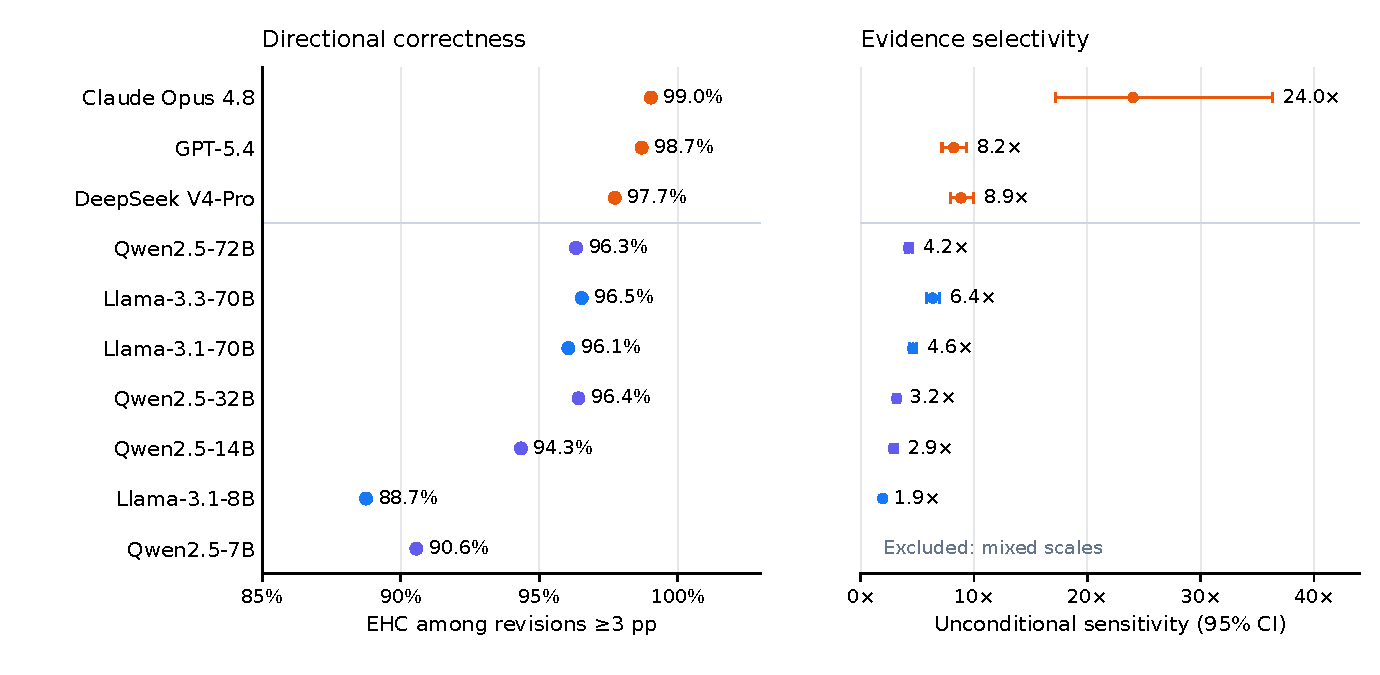
\includegraphics[width=\linewidth]{figures/exp1_ehc_sensitivity_combined.pdf}
\caption{\textbf{Directional consistency and causal selectivity both scale with model size.}
\emph{Left:} Evidence--Hypothesis Consistency rises from $87$--$90\%$ for 7--8B local models
to ${\sim}98$--$99\%$ for frontier systems, with the largest local jump between 8B and 14B.
\emph{Right:} the sensitivity ratio reaches $1.9$--$6.4\times$ for local models and
$8.2$--$24.0\times$ for frontier systems.}
\label{fig:exp1-scale}
\end{figure*}

\paragraph{Finding 3: causal selectivity scales with size but retains a frontier gap.}
The sensitivity ratio (Figure~\ref{fig:exp1-scale}, right) scales monotonically from
$1.9\times$ (Llama~3.1-8B) through $2.7$--$6.4\times$ for local 7--70B models to
$8.2$--$24.0\times$ for frontier.  The frontier gap in selectivity is substantially larger
than the frontier gap in EHC: Llama~3.3-70B nearly matches frontier EHC (.968 vs.\
.978--.990), yet its sensitivity ($6.4\times$) is still well below the frontier range.

Within the frontier tier, Claude Opus~4.8 shows the highest selectivity ($24.0\times$),
followed by DeepSeek V4-Pro ($8.9\times$) and GPT-5.4 ($8.2\times$).  Claude's selectivity
stands far above the other two frontier models despite only a modest EHC lead, indicating
that causal selectivity and directional consistency, while correlated, are not the same
axis.  Per-direction revision magnitudes for all models are in
Appendix~\ref{app:extended-results}.

\paragraph{Finding 4: high consistency is not market imitation.}
As a design validity check we ask how closely each agent's forecasts track the market
(Table~\ref{tab:consistency}, right-hand columns; Figure~\ref{fig:exp1-market}).  We
measure \emph{association} with Spearman rank
correlation $\rho$ between the agent's yes-probability and the Polymarket mid-price, and
\emph{divergence} with mean absolute deviation $\overline{|A{-}M|}$.  We deliberately
avoid a binary, threshold-based agreement statistic: the pool skews low-probability
(64\% of mid-prices below 0.50), so a 0.50 cut would collapse most markets into a single
bucket and discard the probability magnitude.  This is an association control, \emph{not}
calibration---the markets are unresolved, so the mid-price is a proxy, not ground truth.

Association rises monotonically with scale, from $\rho = 0.38$--$0.40$ for the 7--8B
models to $\rho = 0.68$--$0.71$ for the frontier tier; the strongest local model,
Llama~3.3-70B ($\rho = 0.59$), tracks the market about as closely as the frontier
systems.  Crucially, association does not imply imitation: every agent diverges
substantially in magnitude ($\overline{|A{-}M|} = 14$--$21$\,pp), so even the
best-aligned agents are not reproducing prices.  Pairwise inter-agent $\rho$ is in
Appendix~\ref{app:extended-results}.

\paragraph{Interpretation.}
Taken together, the four findings place frontier agents on the \emph{coherence} rung: they
update selectively in the causally relevant direction ($8$--$24\times$), propagate that
update through both output fields (EHC~$\approx$~HFC), and track the market's ranking
without copying its prices (Figure~\ref{fig:exp1-market})---ruling out the surface-matching,
rationalization, and imitation shortcuts of Section~\ref{sec:forecasting-as-inductive}.
Consistency and selectivity both scale with size but unevenly: structural bookkeeping
saturates by 14B, directional consistency climbs through 70B, and causal selectivity
retains the largest frontier gap---with the Llama~3.3-vs-3.1 split at fixed scale
implicating post-training rather than parameter count alone.  These results establish
behavioral coherence but \emph{not} world-model recovery: the counterfactual packets are
deliberately unambiguous and the true latent structure of a real market is unknown, so an
agent could pass every check here while still misrepresenting that structure---precisely the
gap Experiments~2 and~3 close through latent-state inference in synthetic worlds and transfer
across forecasting tasks.

\begin{figure}[t]
\centering
\includegraphics[width=0.62\linewidth]{figures/exp1_market_divergence.pdf}
\caption{
\textbf{Agents track but do not copy the market.}
Agent forecast vs.\ Polymarket price across all pool markets
(${\approx}1{,}050$ market--forecast pairs; frontier in orange, local in faint blue).
Pure market imitation would place every point on the $y=x$ diagonal.  Instead, forecasts
are correlated with the price (pooled Spearman $\rho = 0.67$ frontier, $0.46$ local) but the
frontier least-squares fit is flatter than the diagonal---agents compress toward the interior and
diverge from the market by ${\approx}16$~pp on average---and alignment improves with scale.}
\label{fig:exp1-market}
\end{figure}

Beyond the unambiguous-packet design noted above, Stage~3 disables web search, so agents
cannot flag injected headlines as unverifiable; we revisit both limitations in
Appendix~\ref{app:exp1-limitations}.
